

%% AP Physics MC Questions Archive
%%----------------------------------------


%% Impulse
%%----------------------------------------
\element{ap}{
\begin{question}{impulse-q01}
    A baseball player struck a \SI{1}{\kilo\gram} ball coming inward at \SI{15}{\meter\per\second} giving it a velocity of \SI{35}{\meter\per\second} outward.
    The bat was in contact with the ball for \SI{0.5}{\second}.
    What is the average force the baseball player exerted on the ball?
    \begin{multicols}{3}
    \begin{choices}
        \wrongchoice{\SI{23.33}{\newton}}
        \wrongchoice{\SI{40}{\newton}}
      \correctchoice{\SI{100}{\newton}}
        \wrongchoice{\SI{150}{\newton}}
        \wrongchoice{\SI{350}{\newton}}
    \end{choices}
    \end{multicols}
\end{question}
}

\element{ap}{
\begin{question}{impulse-q02}
    A pool player strikes a \SI{50}{\gram} cue ball with a cue 45 degrees from the plane of the table.
    The stick is in contact with the ball for \SI{0.05}{\second} causing the ball to accelerate to \SI{4}{\meter\per\second}.
    \begin{center}
    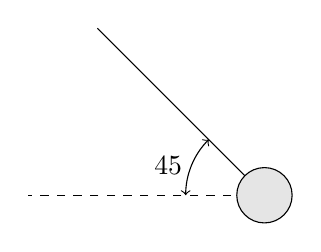
\begin{tikzpicture}
        \draw (0,0) -- (135:3cm);
        \draw[dashed] (0,0) -- (180:3cm);
        \draw[fill=white!90!black] (0,0) circle (1em);
        \draw[<->] (180:1) arc(180:135:1) node[pos=0.5,anchor=east] {\ang{45}};
    \end{tikzpicture}
    \end{center}
    What is the average force exerted on the ball?
    \begin{multicols}{3}
    \begin{choices}
        \wrongchoice{\SI{2.8}{\newton}}
        \wrongchoice{\SI{1.4}{\newton}}
        \wrongchoice{\SI{25}{\newton}}
      \correctchoice{\SI{4}{\newton}}
        \wrongchoice{\SI{2}{\newton}}
    \end{choices}
    \end{multicols}
\end{question}
}

\element{ap}{
\begin{question}{impulse-q03}
    A force of \SI{40}{\newton} acts on an \SI{2}{\kilo\gram} object,
        initially at rest, for \SI{0.5}{\second}.
    Its resulting velocity is:
    \begin{multicols}{3}
    \begin{choices}
        \wrongchoice{\SI{6}{\meter\per\second}}
      \correctchoice{\SI{10}{\meter\per\second}}
        \wrongchoice{\SI{12}{\meter\per\second}}
        \wrongchoice{\SI{20}{\meter\per\second}}
        \wrongchoice{\SI{24}{\meter\per\second}}
    \end{choices}
    \end{multicols}
\end{question}
}

\element{ap}{
\begin{question}{impulse-q04}
    An object accelerates in a straight line from \SI{2}{\meter\per\second} to \SI{8}{\meter\per\second} in \SI{2}{\second} due to an average force of \SI{24}{\newton}.
    The mass of the object is:
    \begin{multicols}{3}
    \begin{choices}
        \wrongchoice{\SI{4}{\kilo\gram}}
        \wrongchoice{\SI{6}{\kilo\gram}}
      \correctchoice{\SI{8}{\kilo\gram}}
        \wrongchoice{\SI{10}{\kilo\gram}}
        \wrongchoice{\SI{12}{\kilo\gram}}
    \end{choices}
    \end{multicols}
\end{question}
}

\element{ap}{
\begin{question}{impulse-q05}
    A ball with mass $m$ is rolled horizontally into a ball and bounces back along its original path at the same speed.
    The change in momentum of the ball is:
    \begin{multicols}{3}
    \begin{choices}
        \wrongchoice{zero}
        \wrongchoice{$\dfrac{1}{2} mv$}
        \wrongchoice{$mv$}
        \wrongchoice{$\dfrac{3}{2} mv$}
      \correctchoice{$2 mv$}
    \end{choices}
    \end{multicols}
\end{question}
}

\element{ap}{
\begin{question}{impulse-q06}
    Two identical dummies are used in a simulation of a car crash.
    Upon impact, the car is moving at \SI{20}{\meter\per\second}.
    Dummy $A$ comes to rest in \SI{20}{\milli\second}.
    Dummy $B$ has an airbag, and comes to rest in \SI{2}{\second}.
    What is the ratio of the force felt by Dummy $A$ to that felt by Dummy $B$?
    \begin{multicols}{3}
    \begin{choices}
        \wrongchoice{$1:100$}
        \wrongchoice{$1:10$}
        \wrongchoice{$10:1$}
      \correctchoice{$100:1$}
        \wrongchoice{$1000:1$}
    \end{choices}
    \end{multicols}
\end{question}
}

\element{ap}{
\begin{question}{impulse-q07}
    If $L$, $M$ and $T$ denote the dimensions of length,
        mass, and time, respectively,
        what are the dimensions of impulse?
    \begin{multicols}{3}
    \begin{choices}
      \correctchoice{$\dfrac{\mathrm{ML}}{\mathrm{T}}$}
        \wrongchoice{$\dfrac{\mathrm{ML}}{\mathrm{T}^2}$}
        \wrongchoice{$\dfrac{\mathrm{LT}}{\mathrm{M}}$}
        \wrongchoice{$\dfrac{\mathrm{LT}^2}{\mathrm{M}}$}
        \wrongchoice{$\dfrac{\mathrm{MT}^2}{\mathrm{L}}$}
    \end{choices}
    \end{multicols}
\end{question}
}

\element{ap}{
\begin{question}{impulse-q08}
    A child on a frictionless surface pushes a box in the $x$-direction
        (on the same frictionless surface).
    The box slides along the surface until it strikes a wall,
        staying in contact with the wall for \SI{0.2}{\second} imparting an impulse of \SI{16}{\kilo\gram\meter\per\second} before coming to rest.
    The child accelerates at a rate of \SI{1.25}{\meter\per\second\squared} in the $-x$ direction.
    What is the mass of the child?
    \begin{multicols}{3}
    \begin{choices}
        \wrongchoice{\SI{50}{\kilo\gram}}
        \wrongchoice{\SI{56}{\kilo\gram}}
        \wrongchoice{\SI{60}{\kilo\gram}}
      \correctchoice{\SI{64}{\kilo\gram}}
        \wrongchoice{\SI{80}{\kilo\gram}}
    \end{choices}
    \end{multicols}
\end{question}
}

\element{ap}{
\begin{question}{impulse-q09}
    Base your answer to the following question on the graph below.
    \begin{center}
    \begin{tikzpicture}
        \begin{axis}[
            axis y line=left,
            axis x line=bottom,
            axis line style={->},
            xlabel={time},
            x unit=\si{\second},
            xtick={1,2,3},
            ylabel={force},
            y unit=\si{\newton},
            ytick={10,20,30},
            xmin=0,xmax=3.2,
            ymin=0,ymax=32,
            grid=major,
            width=0.8\columnwidth,
            height=0.5\columnwidth,
            very thin,
        ]
        \addplot[line width=1pt,mark=\empty] plot coordinates {(0,0) (3,30)};
        \end{axis}
    \end{tikzpicture}
    \end{center}
    What is the impulse imparted by the force during this interval?
    \begin{multicols}{3}
    \begin{choices}
        \wrongchoice{\SI{10}{\newton\second}}
        \wrongchoice{\SI{30}{\newton\second}}
      \correctchoice{\SI{45}{\newton\second}}
        \wrongchoice{\SI{60}{\newton\second}}
        \wrongchoice{\SI{90}{\newton\second}}
    \end{choices}
    \end{multicols}
\end{question}
}

\element{ap}{
\begin{question}{impulse-q10}
    A spring of constant \SI{50}{\newton\per\meter} is compressed \SI{20}{\centi\meter} by a \SI{0.5}{\kilo\gram} mass.
    If the spring is released,
        what is the impulse imparted to the mass by the spring?
    \begin{multicols}{3}
    \begin{choices}
        \wrongchoice{\SI{0.5}{\kilo\gram\meter\per\second}}
        \wrongchoice{\SI{0.9}{\kilo\gram\meter\per\second}}
      \correctchoice{\SI{1}{\kilo\gram\meter\per\second}}
        \wrongchoice{\SI{1.5}{\kilo\gram\meter\per\second}}
        \wrongchoice{\SI{1.8}{\kilo\gram\meter\per\second}}
    \end{choices}
    \end{multicols}
\end{question}
}

\newcommand{\apImpulseQEleven}{
\begin{tikzpicture}
    \begin{axis}[
        axis y line=left,
        axis x line=bottom,
        axis line style={->},
        xlabel={time},
        x unit=\si{\second},
        xtick={1,2,3,4,5},
        ylabel={force},
        y unit=\si{\newton},
        ytick={10,20,30,40},
        xmin=0,xmax=5.5,
        ymin=0,ymax=45,
        grid=major,
        width=0.8\columnwidth,
        height=0.5\columnwidth,
        very thin,
    ]
    \addplot[line width=1pt,mark=\empty] plot coordinates {(0,0) (2,35) (4,35) (5,0)};
    \end{axis}
\end{tikzpicture}
}

%% NOTE: impulse-q11A, momentum at 4s
%% NOTE: impulse-q12A, kinetic energy at 4s
\element{ap}{
\begin{question}{impulse-q11}
    %Base your answers to questions 11 and 12 on the force-time graph below,
    The force-time graph below is for a \SI{3.5}{\kilo\gram} object,
        starting from rest, moving in a straight line.
    \begin{center}
        \apImpulseQEleven
    \end{center}
    %% Start question
    What is the object's momentum at \SI{3.0}{\second}?
    \begin{multicols}{3}
    \begin{choices}
        \wrongchoice{\SI{35}{\kilo\gram\meter\per\second}}
      \correctchoice{\SI{50}{\kilo\gram\meter\per\second}}
        \wrongchoice{\SI{70}{\kilo\gram\meter\per\second}}
        \wrongchoice{\SI{100}{\kilo\gram\meter\per\second}}
        \wrongchoice{\SI{105}{\kilo\gram\meter\per\second}}
    \end{choices}
    \end{multicols}
\end{question}
}

\element{ap}{
\begin{question}{impulse-q12}
    %Base your answers to questions 11 and 12 on the force-time graph below,
    The force-time graph below is for a \SI{3.5}{\kilo\gram} object,
        starting from rest, moving in a straight line.
    \begin{center}
        \apImpulseQEleven
    \end{center}
    %% Start question
    What is the kinetic energy of the particle after \SI{2.0}{\second}?
    \begin{multicols}{3}
    \begin{choices}
        \wrongchoice{\SI{35}{\joule}}
        \wrongchoice{\SI{70}{\joule}}
        \wrongchoice{\SI{140}{\joule}}
      \correctchoice{\SI{175}{\joule}}
        \wrongchoice{\SI{210}{\joule}}
    \end{choices}
    \end{multicols}
\end{question}
}

\newcommand{\apImpulseQThirteen}{
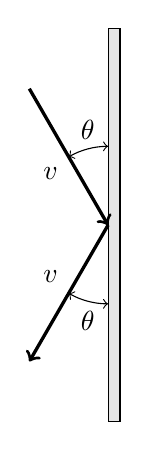
\begin{tikzpicture}
    \draw[fill=white!90!black] (0,-2.5) rectangle (1ex,2.5);
    \draw[very thick,<-] (0,0) -- (120:2) node[pos=0.5,anchor=north east] {$v$};
    \draw[very thick,->] (0,0) -- (240:2) node[pos=0.5,anchor=south east] {$v$};
    \draw[<->] (90:1) arc(90:120:1) node[pos=0.5,anchor=south] {$\theta$};
    \draw[<->] (270:1) arc(270:240:1) node[pos=0.5,anchor=north] {$\theta$};
\end{tikzpicture}
}

\element{ap}{
\begin{question}{impulse-q13}
    A ball of mass $m$ rebounds from a wall with the same speed $v$ as it had initially,
        as shown below.
    \begin{center}
        \apImpulseQThirteen
    \end{center}
    The magnitude of the impulse delivered to the wall is:
    \begin{multicols}{3}
    \begin{choices}
        \wrongchoice{zero}
        \wrongchoice{$mv$}
        \wrongchoice{$2mv$}
        \wrongchoice{$2mv\cos\theta$}
      \correctchoice{$2mv\sin\theta$}
    \end{choices}
    \end{multicols}
\end{question}
}

\element{ap}{
\begin{question}{impulse-q14}
    A ball of mass $m$ rebounds from a wall with the same speed $v$ as it had initially,
        as shown below.
    \begin{center}
        \apImpulseQThirteen
    \end{center}
    A ball of mass $m$ bounces off of a wall with the same speed $v$ that it had initially.
    If the ball was in contact with the wall for a time $t$ and during this time an average force $F$ was applied to it,
        then the angle made between the wall and the ball's trajectory is:
    \begin{multicols}{2}
    \begin{choices}
        \wrongchoice{$\dfrac{Ft}{mv}$}
        \wrongchoice{$\cos^{-1}\left(\dfrac{Ft}{mv}\right)$}
        \wrongchoice{$\cos^{-1}\left(\dfrac{Ft}{2mv}\right)$}
        \wrongchoice{$\sin^{-1}\left(\dfrac{Ft}{mv}\right)$}
      \correctchoice{$\sin^{-1}\left(\dfrac{Ft}{2mv}\right)$}
    \end{choices}
    \end{multicols}
\end{question}
}

\element{ap}{
\begin{questionmult}{impulse-q15}
    An object is in freefall on Earth.
    Which of the following statements is/are true?
    \begin{choices}
        %% also correct
      \correctchoice{The object is gaining an equal amount of momentum for each second it is in free fall.}
        \wrongchoice{The object is gaining an equal amount of momentum for each meter it falls.}
        %% orig correct answer
      \correctchoice{The object is gaining an equal amount of kinetic energy for each meter it falls.}
        \wrongchoice{The object is gaining an equal amount of kinetic energy for each second it falls.}
        \wrongchoice{The object is gaining an equal amount of speed for each meter it falls.}
    \end{choices}
\end{questionmult}
}

\element{ap}{
\begin{question}{impulse-q16}
    An object of mass $M$ is dropped from rest off of a cliff.
    %After \SI{5}{\second} it is a distance $L$ from its initial location,
    After time $t$ it is a distance $L$ from its initial location,
        what is its momentum?
    \begin{multicols}{3}
    \begin{choices}
        \wrongchoice{$t^2 Mg$}
        \wrongchoice{$3t Mg$}
      \correctchoice{$tMg$}
        \wrongchoice{$Mg$}
        \wrongchoice{$MgL$}
    \end{choices}
    \end{multicols}
\end{question}
}

\element{ap}{
\begin{question}{impulse-q17}
    A mass of \SI{10}{\kilo\gram} was accelerated from rest to \SI{10}{\meter\per\second} in 1 second.
    What is the impulse this mass experienced?
    \begin{multicols}{3}
    \begin{choices}
        \wrongchoice{\SI{10}{\newton\second}}
      \correctchoice{\SI{100}{\newton\second}}
        \wrongchoice{\SI{50}{\newton\second}}
        \wrongchoice{\SI{25}{\newton\second}}
        \wrongchoice{\SI{12.5}{\newton\second}}
    \end{choices}
    \end{multicols}
\end{question}
}

%% Graphic is technically not needed
%\newcommand{\apImpulseQEighteen}{
%}

\element{ap}{
\begin{question}{impulse-q18}
    %%Base your answers to questions 18 and 19 on the following information.
    A car of mass \SI{1500}{\kilo\gram} traveling at a velocity of \SI{25}{\meter\per\second} crashes through a roadblock for \SI{4}{\second} and continues on the road traveling at \SI{5}{\meter\per\second}.
    %% start question
    What is the impulse of the roadblock on the car?
    \begin{multicols}{2}
    \begin{choices}
        \wrongchoice{\SI{500}{\newton\second}}
        \wrongchoice{\SI{2 500}{\newton\per\second}}
        \wrongchoice{\SI{6 000}{\kilo\gram\meter\per\second}}
        \wrongchoice{\SI{15 000}{\kilo\gram\meter\per\second}}
      \correctchoice{\SI{30 000}{\kilo\gram\meter\per\second}}
    \end{choices}
    \end{multicols}
\end{question}
}

\element{ap}{
\begin{question}{impulse-q19}
    %%Base your answers to questions 18 and 19 on the following information.
    A car of mass \SI{1500}{\kilo\gram} traveling at a velocity of \SI{25}{\meter\per\second} crashes through a roadblock for \SI{4}{\second} and continues on the road traveling at \SI{5}{\meter\per\second}.
    %% start question
    What is the car's change in kinetic energy?
    \begin{multicols}{2}
    \begin{choices}
        \wrongchoice{\SI{300 000}{\joule}}
      \correctchoice{\SI{450 000}{\joule}}
        \wrongchoice{\SI{75 000}{\joule}}
        \wrongchoice{\SI{45 000}{\joule}}
        \wrongchoice{\SI{30 000}{\joule}}
    \end{choices}
    \end{multicols}
\end{question}
}

\element{ap}{
\begin{question}{impulse-q20}
    An object with a mass of \SI{4}{\kilo\gram} has a kinetic energy of \SI{18}{\joule}.
    The object's linear momentum is:
    \begin{multicols}{2}
    \begin{choices}
        \wrongchoice{\SI{6}{\kilo\gram\meter\per\second}}
        \wrongchoice{\SI{9}{\kilo\gram\meter\per\second}}
      \correctchoice{\SI{12}{\kilo\gram\meter\per\second}}
        \wrongchoice{\SI{20}{\kilo\gram\meter\per\second}}
        \wrongchoice{\SI{72}{\kilo\gram\meter\per\second}}
    \end{choices}
    \end{multicols}
\end{question}
}

\element{ap}{
\begin{question}{impulse-q21}
    An object has a linear momentum of \SI{10}{\kilo\gram\meter\per\second} and a kinetic energy of \SI{25}{\joule}.
    It's mass is equal to:
    \begin{multicols}{2}
    \begin{choices}
      \correctchoice{\SI{2}{\kilo\gram}}
        \wrongchoice{\SI{2.5}{\kilo\gram}}
        \wrongchoice{\SI{5}{\kilo\gram}}
        \wrongchoice{\SI{10}{\kilo\gram}}
        \wrongchoice{Cannot be determined from the information provided.}
    \end{choices}
    \end{multicols}
\end{question}
}

\element{ap}{
\begin{question}{impulse-q22}
    An object has its momentum increased by \SI{6}{\kilo\gram\meter\per\second} in \SI{0.3}{\second}.
    The force applied to the object in this time was:
    \begin{multicols}{2}
    \begin{choices}
        \wrongchoice{\SI{2}{\kilo\gram\meter\per\second\squared}}
        \wrongchoice{\SI{5}{\kilo\gram\meter\per\second\squared}}
        \wrongchoice{\SI{10}{\kilo\gram\meter\per\second\squared}}
      \correctchoice{\SI{20}{\kilo\gram\meter\per\second\squared}}
        \wrongchoice{\SI{25}{\kilo\gram\meter\per\second\squared}}
    \end{choices}
    \end{multicols}
\end{question}
}

\element{ap}{
\begin{questionmult}{impulse-q23}
    A ball with mass $m$ collides with another,
        larger ball, with mass $M$.
    Which of the following is/are true about the collision?
    \begin{choices}
        \wrongchoice{The larger ball will experience a greater impulse than the smaller ball.}
        \wrongchoice{The magnitude of the force felt by the small ball from the large ball will be greater than the magnitude of the force felt by the large ball from the small ball.}
      \correctchoice{The magnitude of the acceleration of the small ball will be greater than the magnitude of the acceleration of the large ball.}
    \end{choices}
\end{questionmult}
}

\element{ap}{
\begin{question}{impulse-q24}
    Two objects collide, one being more massive than the other.
    The magnitude of which of the following would necessarily be greater for the smaller mass than for the larger?
    \begin{choices}
        \wrongchoice{impulse}
      \correctchoice{acceleration}
        \wrongchoice{change in momentum}
        \wrongchoice{force}
        \wrongchoice{change in kinetic energy}
    \end{choices}
\end{question}
}

\element{ap}{
\begin{question}{impulse-q25}
    Airbags inflating in a motor vehicle accident protect the passengers because
    \begin{choices}
        \wrongchoice{The increased area of the airbag reduces the force on the passenger.}
        \wrongchoice{The change in the momentum of the passenger is reduced by the presence of the airbag.}
      \correctchoice{The airbag increases the time of impact, decreasing the average force on the passenger.}
        \wrongchoice{The airbag decreases the time of impact, reducing the impulse delivered to the passenger.}
        \wrongchoice{The impulse delivered to the passenger is reduced by the presence of the airbag.}
    \end{choices}
\end{question}
}

\element{ap}{
\begin{question}{impulse-q26}
    An experiment is performed with two trials.
    In the first, an object has a force $F$ applied to it in a time $t$.
    In the second, $F$ is applied to the same object in time $2t$.
    The ratio between the acceleration of the object in the first trial to the second is
    \begin{multicols}{3}
    \begin{choices}
        \wrongchoice{$1:4$}
        \wrongchoice{$1:2$}
        \wrongchoice{$1:1$}
      \correctchoice{$2:1$}
        \wrongchoice{$4:1$}
    \end{choices}
    \end{multicols}
\end{question}
}

\element{ap}{
\begin{questionmult}{impulse-q27}
    %Base your answer to the following question on the graphs below,
    %    which plot the velocity of a particle with respect to time.
    In which of these cases is the object's rate of change of momentum constant?
    \begin{multicols}{2}
    \begin{choices}
        \AMCboxDimensions{down=-1.5em}
        \correctchoice{
            \begin{tikzpicture}
                \begin{axis}[
                    axis y line=left,
                    axis x line=bottom,
                    axis line style={->},
                    xlabel={time},
                    xtick=\empty,
                    ylabel={velocity},
                    ytick=\empty,
                    xmin=0,xmax=11,
                    ymin=0,ymax=11,
                    width=0.95\columnwidth,
                    very thin,
                ]
                \addplot[line width=1pt,domain=0:10]{x};
                \end{axis}
            \end{tikzpicture}
        }
        \correctchoice{
            \begin{tikzpicture}
                \begin{axis}[
                    axis y line=left,
                    axis x line=bottom,
                    axis line style={->},
                    xlabel={time},
                    xtick=\empty,
                    ylabel={velocity},
                    ytick=\empty,
                    xmin=0,xmax=11,
                    ymin=0,ymax=11,
                    width=0.95\columnwidth,
                    very thin,
                ]
                \addplot[line width=1pt,domain=0:10]{8};
                \end{axis}
            \end{tikzpicture}
        }
        \wrongchoice{
            \begin{tikzpicture}
                \begin{axis}[
                    axis y line=left,
                    axis x line=bottom,
                    axis line style={->},
                    xlabel={time},
                    xtick=\empty,
                    ylabel={velocity},
                    ytick=\empty,
                    xmin=0,xmax=11,
                    ymin=0,ymax=11,
                    width=0.95\columnwidth,
                    very thin,
                ]
                \addplot[line width=1pt,domain=0:10]{0.1*x*x};
                \end{axis}
            \end{tikzpicture}
        }
    \end{choices}
    \end{multicols}
\end{questionmult}
}

\element{ap}{
\begin{question}{impulse-q28}
    A cannonball with mass \SI{25}{\kilo\gram} is initially at rest.
    It is fired out of a cannon with a speed of \SI{40}{\meter\per\second} in a direction \ang{30} above the horizontal.
    The magnitude of the impulse imparted to the cannonball by the cannon is most nearly
    \begin{multicols}{2}
    \begin{choices}
        \wrongchoice{\SI{5 000}{\newton\second}}
        \wrongchoice{$\num{1000}\sqrt{3}\,\si{\newton\second}$}
      \correctchoice{\SI{1 000}{\newton\second}}
        \wrongchoice{$\num{10 000}\sqrt{3}\,\si{\newton\second}$}
        \wrongchoice{\SI{20 000}{\newton\second}}
    \end{choices}
    \end{multicols}
\end{question}
}

\element{ap}{
\begin{question}{impulse-q29}
    Two skaters are on ice with negligible friction.
    One skater has a mass $m$, the other, a mass $M$ where $M>m$.
    The skaters are at rest when they simultaneously push each other horizontally.
    Which is true about their subsequent motion?
    \begin{choices}
        \wrongchoice{The center of mass of the two-skater system will move in the direction of the less massive skater.}
        \wrongchoice{The more massive person will have a greater initial acceleration than the less massive.}
        \wrongchoice{The velocities of both skaters will be equal.}
        \wrongchoice{The speeds of both skaters will be equal.}
      \correctchoice{The momenta of the two skaters are equal in magnitude.}
    \end{choices}
\end{question}
}


\endinput


